% opis interfejsu graficznego aplikacji

\section{Interfejs graficzny}
Wygląd interfejsu graficznego aplikacji przedstawiony jest na rysunku \ref{fig:gui}.

\begin{figure}
 \begin{center} 
  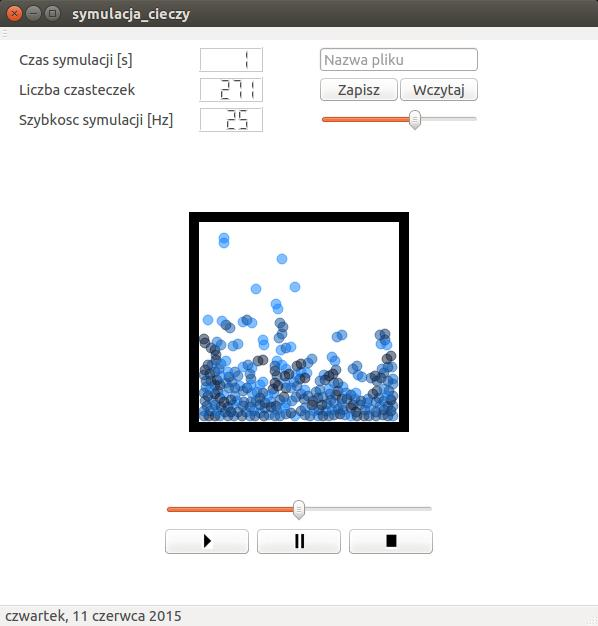
\includegraphics{./rysunki/new_gui.jpeg} 
 \end{center}
 \caption{Interfejs graficzny aplikacji}
 \label{fig:gui} 
\end{figure}

W centralnej części aplikacji widoczny jest jej główny element, a zatem zbiornik z~cząsteczkami. Pod nim znajduje się slider pozwalający na przechylanie zbiornika.

Użytkownik za pomocą trzech przycisków umiejscowionych na dole ekranu może sterować symulacją, a mianowicie ją: uruchomić, zamrozić lub zatrzymać.  

W lewej górnej części okienka znajdują się elementy pozwalające śledzić (i~modyfikować) parametry symulacji: jej czas trwania, symulowaną liczbę cząsteczek oraz szybkość odświeżania wizualizacji. Umiejscowione są tam również przyciski i pole tekstowe pozwalające na zapisanie bądź wczytanie stanu symulacji.

Na widocznej w dole ekranu belce statusowej wyświetlana jest aktualna data.

W pasku menu dostępne są opcje: zapisu symulacji oraz zamknięcia aplikacji.

Interfejs graficzny jest odpowiednio modyfikowany przy zmianie wymiarów okienka.